\clearpage\chapter{The Type Inferencing Model}

Three sections of this dissertation are devoted to type inferencing:
two chapters and an appendix. This chapter develops a theoretical
model of type inferencing for Icon. For simplicity, it ignores some
features of the language. This chapter presents intuitive arguments
for the correctness of the formal model. Chapter 19 describes the
actual implementation of type inferencing in the Icon compiler. The
implementation handles the full Icon language and, for pragmatic
reasons, differs from the theoretical model in some details.


This chapter starts with the motivation for performing type
inferencing. It then describes the concept of \textit{abstract
interpretation}. This concept is used as a tool in this chapter to
develop a type inferencing system from Icon's semantics. This chapter
gives an intuitive presentation of this development process before
presenting the formal models of abstract semantics for Icon. The most
abstract of the formal models is the type inferencing system.

\section[15.1 Motivation]{15.1 Motivation}

Variables in the Icon programming language are untyped. That is, a
variable may take on values of different types as the execution of a
program proceeds. In the following example, \texttt{x} contains a
string after the read (if the read succeeds), but it is then assigned
an integer or real, provided the string can be converted to a numeric
type.

\goodbreak
\begin{iconcode}
x := read()\\
if numeric(x) then x +:= 4\\
\end{iconcode}


In general, it is impossible to know the type of an operator's
operands at translation time, so some type checking must be done at
run time. This type checking may result in type conversions, run-time
errors, or the selection among polymorphous operations (for example,
the selection of integer versus real addition). In the Icon
interpreter system, all operators check all of their operands at run
time. This incurs significant overhead.

Much of this run-time type checking is unnecessary. An examination of
typical Icon programs reveals that the types of most variables remain
consistent throughout execution (except for the initial null value)
and that these types can often be determined by inspection. Consider

\goodbreak
\begin{iconcode}
if x := read() then\\
\>y := x || ";"\\
\end{iconcode}


Clearly both operands of {\textbar}{\textbar} are strings so no
checking or conversion is needed.

The goal of a type inferencing system is to determine what types
variables may take on during the execution of a program. It associates
with each variable usage a set of the possible types of values that
variable might have when execution reaches the usage. This set may be
a conservative estimate (overestimate) of the actual set of possible
types that a variable may take on because the actual set may not be
computable, or because an analysis to compute the actual set may be
too expensive. However, a good type inferencing system operating on
realistic programs can determine the exact set of types for most
operands and the majority of these sets in fact contain single types,
which is the information needed to generate code without type
checking. The Icon compiler has an effective type inferencing system
based on data flow analysis techniques.

\section[15.2 Abstract Interpretation ]{15.2 Abstract Interpretation }

Data flow analysis can be viewed as a form of abstract interpretation
[.absintrp.]. This can be particularly useful for understanding type
inferencing. A ``concrete'' interpreter for a language implements the
standard (operational) semantics of the language, producing a sequence
of states, where a state consists of an execution point, bindings of
program variables to values, and so forth. An abstract interpreter
does not implement the semantics, but rather computes information
related to the semantics. For example, an abstract interpretation may
compute the sign of an arithmetic expression rather than its
value. Often it computes a ``conservative'' estimate for the property
of interest rather than computing exact information. Data flow
analysis is simply a form of abstract interpretation that is
guaranteed to terminate. This chapter presents a sequence of
approximations to Icon semantics, culminating in one suitable for type
inferencing.

Consider a simplified operational semantics for Icon, consisting only
of program points (with the current execution point maintained in a
program counter) and variable bindings (maintained in an
environment). As an example of these semantics, consider the following
program. Four program points are annotated with numbers using comments
(there are numerous intermediate points not annotated).

\goodbreak
\begin{iconcode}
procedure main()\\
local s, n\\
\\
\>\# 1:\\
\>s := read()\\
\>\# 2:\\
\>every n := 1 to 2 do \{\\
\>\>\# 3:\\
\>\>write(s[n])\\
\>\>\}\\
\>\# 4:\\
end\\
\end{iconcode}


If the program is executed with an input of \texttt{abc}, the following states
are included in the execution sequence (only the annotated points are
listed). States are expressed in the form \textit{program point}:
\textit{environment}.

\goodbreak
\begin{specialcode}{}
\>\>1: [\texttt{s} = null, \texttt{n} = null]\\
\>\>2: [\texttt{s} = "\texttt{abc}", \texttt{n} = null]\\
\>\>3: [\texttt{s} = "\texttt{abc}", \texttt{n} = 1]\\
\>\>3: [\texttt{s} = "\texttt{abc}", \texttt{n} = 2]\\
\>\>4: [\texttt{s} = "\texttt{abc}", \texttt{n} = 2]\\
\end{specialcode}


It is customary to use the \textit{collecting semantics} of a language
as the first abstraction (approximation) to the standard semantics of
the language. The collecting semantics of a program is defined in
Cousot and Cousot [.absintrp.]  (they use the term \textit{static
semantics}) to be an association between program points and the sets
of environments that can occur at those points during all possible
executions of the program.

Once again, consider the previous example. In general, the input to
the program is unknown, so the read function is assumed to be capable
of producing any string. Representing this general case, the set of
environments (once again showing only variable bindings) that can
occur at point 3 is

\goodbreak
\begin{specialcode}{}
\>\>[\texttt{s} = "", \texttt{n} = 1],\\
\>\>[\texttt{s} = "", \texttt{n} = 2],\\
\>\>[\texttt{s} = "a", \texttt{n} = 1],\\
\>\>[\texttt{s} = "a", \texttt{n} = 2],\\
\>\>\>\ \ldots\\
\>\>[\texttt{s} = "\texttt{abcd}", \texttt{n} = 1],\\
\>\>[\texttt{s} = "\texttt{abcd}", \texttt{n} = 2],\\
\>\>\> \ldots\\
\end{specialcode}


A type inferencing abstraction further approximates this information,
producing an association between each variable and a type at each
program point. The actual type system chosen for this abstraction must
be based on the language and the use to which the information is
put. The type system used here is based on Icon's run-time type
system. For structure types, the system used retains more information
than a simple use of Icon's type system would retain; this is
explained in detail later. For atomic types, Icon's type system is
used as is. For point 3 in the preceding example the associations
between variables and types are

\begin{specialcode}{}
\>\>[\texttt{s} = string, \texttt{n} = integer]\\
\end{specialcode}

The type inferencing system presented in this chapter is best
understood as the culmination of a sequence of abstractions to the
semantics of Icon, where each abstraction discards certain
information. For example, the collecting semantics discards sequencing
information among states; in the preceding program, collecting
semantics determine that, at point 3, states may occur with \texttt{n}
equal to 1 and with \texttt{n} equal to 2, but does not determine the
order in which they must occur. This sequencing information is
discarded because desired type information is a static property of the
program.


The first abstraction beyond the collecting semantics discards dynamic
control flow information for goal directed evaluation. The second
abstraction collects, for each variable, the value associated with the
variable in each environment. It discards information such as,
``\texttt{x} has the value 3 when \texttt{y} has the value 7'',
replacing it with ``\texttt{x} may have the value 3 sometime
and \texttt{y} may have the value 7 sometime.''. It effectively
decouples associations between variables.

This second abstraction associates a set of values with a variable,
but this set may be any of an infinite number of sets and it may
contain an infinite number of values. In general, this precludes
either a finite computation of the sets or a finite representation of
them. The third abstraction defines a type system that has a finite
representation.  This abstraction discards information by increasing
the set associated with a variable (that is, making the set less
precise) until it matches a type. This third model can be implemented
with standard iterative data flow analysis techniques.

This chapter assumes that an Icon program consists of a single
procedure and that all invocations are to built-in functions. It also
assumes that there are no co-expressions beyond the main
co-expression. See Chapter 19 for information on how to extend the
abstractions to multiple procedures and multiple co-expressions.


\section[15.3 Collecting Semantics]{15.3 Collecting Semantics}

The collecting semantics of an Icon program is defined in terms of a
\textit{flow graph} of the program. A flow graph is a directed graph
used to represent the flow of control in a program. Nodes in the graph
represent the executable primitives in the program. An edge exists
from node \textbf{A} to node \textbf{B} if it is possible for
execution to pass directly from the primitive represented by node
\textbf{A} to the primitive represented by node \textbf{B}. Cousot and
Cousot [.absintrp.] prove that the collecting semantics of a program
can be represented as the least fixed point of a set of equations
defined over the edges of the program's flow graph. These equations
operate on sets of environments.

For an example of a flow graph, consider the Icon program 

\goodbreak
\begin{iconcode}
procedure main()\\
\>every write(1 to 3)\\
end\\
\end{iconcode}

\noindent
The diagram below on the left shows the abstract syntax tree for this
procedure, including the implicit \texttt{fail} at the end of the
procedure. The invoke node in the syntax tree represents procedure
invocation. Its first argument must evaluate to the procedure to be
invoked; in this case the first argument is the global variable
\texttt{write}. The rest of the arguments are used as the arguments to the
procedure. \texttt{pfail} represents procedure failure (as opposed to
expression failure within a procedure). Nodes corresponding to
operations that produce values are numbered for purposes explained
below.

A flow graph can be derived from the syntax tree. This is shown on the right. 

\begin{picture}(400,250)
%\put(0,0){\graphpaper{40}{25}}
\put(0,0){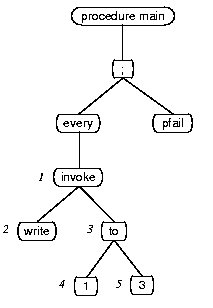
\includegraphics[width=2.4in,height=3.4in]{kw/figure3-1.png}}
\put(200,20){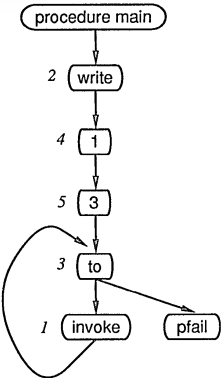
\includegraphics[width=2.2in,height=3.1in]{kw/figure3-2.png}}
\end{picture}

The node labeled procedure main is the \textit{start node} for the
procedure; it performs any necessary initializations to establish the
execution environment for the procedure. The edge from \texttt{invoke}
to \texttt{to} is a resumption path induced by the control structure
\texttt{every}. The path from \texttt{to} to \texttt{pfail} is the
failure path for \texttt{to}. It is a forward execution path rather
than a resumption path because the compound expression (indicated by
\texttt{;}) limits backtracking out of its left-hand sub-expression.
Chapter 19 describes how to determine the edges of the flow graph for
an Icon program.

Both the standard semantics and the abstract semantics must deal with
the intermediate results of expression evaluation.  A
temporary-variable model is used because it is more convenient for
this analysis than a stack model. This decision is unrelated to the
use of a temporary-variable model in the compiler. This analysis uses
a trivial assignment of temporary variables to intermediate
results. Temporary variables are not reused. Each node that produces a
result is assigned some temporary variable \textit{ri} in the
environment. Assuming that temporary variables are assigned to the
example according to the node numbering, the \texttt{to} operation has
the effect of

\iconline{\>\>\ttit{r3} := \ttit{r4} to \ttit{r5} }

\noindent
Expressions that represent alternate computations must be assigned the
same temporary variable, as in the following example for the
subexpression \texttt{x := ("a" {\textbar} "b")}. The syntax tree
below on the left and the flow graph are shown on the right.

\begin{picture}(400,180)
%\put(0,0){\graphpaper{40}{18}}
\put(0,0){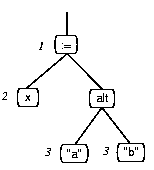
\includegraphics[width=2.2492in,height=2.2398in]{kw/figure3-3.png}}
\put(200,0){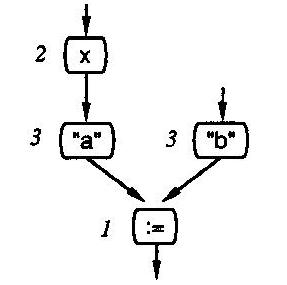
\includegraphics[width=2.4154in,height=2.3in]{kw/figure3-4.png}}
\end{picture}

The \texttt{if} and \texttt{case} control structures are handled
similarly. In addition to temporary variables for intermediate
results, some generators may need additional temporary variables to
hold internal states during suspension. It is easy to devise a scheme
to allocate them where they are needed; details are not presented
here. The syntax tree is kept during abstract interpretation and used
to determine the temporary variables associated with an operation and
its operands.

The equations that determine the collecting semantics of the program
are derived directly from the standard semantics of the language. The
set of environments on an edge of the flow graph is related to the
sets of environments on edges coming into the node at the head of this
edge. This relationship is derived by applying the meaning of the node
(in the standard semantics) to each of the incoming environments.

It requires a rather complex environment to capture the full
operational semantics (and collecting semantics) of a language like
Icon. For example, the environment needs to include a representation
of the external file system.  However, later abstractions only use the
fact that the function \texttt{read} produces strings. This discussion
assumes that it is possible to represent the file system in the
environment, but does not give a representation. Other complexities of
the environment are discussed later. For the moment, examples only
show the bindings of variables to unstructured (atomic) values.

As an example of environments associated with the edges of a flow
graph, consider the assignment at the end of the following code
fragment. The comments in the if expression are assertions that are
assumed to hold at those points in the example.

\goodbreak
\begin{iconcode}
\>if x = 7 then \{\\
\>\>...\\
\>\>\# x is 7 and y is 3\\
\>\>\}\\
\>else \{\\
\>\>...\\
\>\>\# (x is null and y is 1) or (x is "abc" and y is 2)\\
\>\>\}\\
\>x := y + 2\\
\end{iconcode}


Because of the preceding \texttt{if} expression, there are two paths
reaching the assignment. The diagram below shows the flow graph and
accompanying environments for the expression; the diagram ignores the
fact that the assignment expression requires several primitive
operations to implement.


 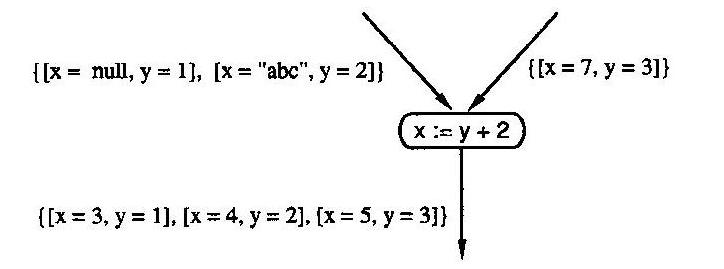
\includegraphics[width=6.0in,height=2.1in]{kw/figure3-5.png}  


For a conditional expression, an incoming environment is propagated to
the path that it would cause execution to take in the standard
semantics. This requires distinguishing the paths to be taken on
failure (backtracking paths) from those to be taken on success. The
following diagram shows an example of this.

{\centering  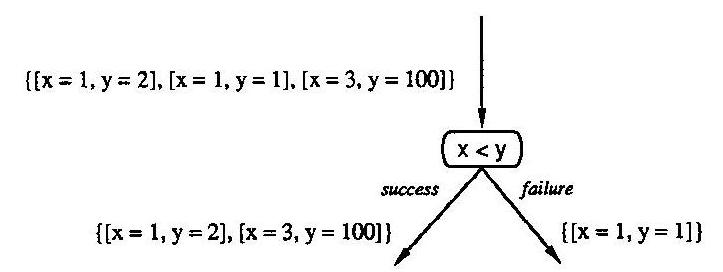
\includegraphics[width=5.3992in,height=2.2299in]{kw/figure3-6.png} \par}

In general there may be several possible backtracking paths. The
environments in the standard and collecting semantics need to include
a stack of current backtracking points and control flow information,
and the flow graph needs instructions to maintain this stack. The Icon
interpreter system described in Part I is an example of how this
information can be maintained. However, the first abstraction to the
collecting semantics eliminates the need for this information, so the
information is not presented in detail here.

\section{Model 1: Eliminating Control Flow Information}

The first abstraction involves taking the union of the environments
propagated along all the failure paths from a node in the collecting
semantics and propagating that union along each of the failure paths
in the new abstraction. This abstraction eliminates the stack of
backtracking points from the environment.

A more formal definition for this model requires taking a closer look
at Icon data values, especially those values with internal
structure. In order to handle Icon data objects with pointer
semantics, an environment needs more than variable bindings. This fact
is important to type inferencing. The problem is handled by including
two components in the environment. The first is the \textit{store},
which maps variables to values. Variables include \textit{named}
variables, \textit{temporary} variables, and \textit{structure}
variables. Named variables correspond to program
identifiers. Temporary variables hold intermediate results as
discussed above. Structure variables are elements of structures such
as lists. Note that the sets of named variables and temporary
variables are each finite (based on the assumption that a program
consists of a single non-recursive procedure; as mentioned earlier,
this assumption is removed in Chapter 19), but for some
non-terminating programs, the set of structure variables may be
infinite.  \textit{Program} variables include both named variables and
structure variables but not temporary variables.

Values include atomic data values such as integers, csets, and
strings. They also include \textit{pointers} that reference objects
with pointer semantics. In addition to the values just described,
temporary variables may contain references to program variables. These
\textit{variable references} may be used by assignments to update the
store or they may be dereferenced by other operations to obtain the
values stored in the variables.

The second part of the environment is the \textit{heap}. It maps
pointers to the corresponding data objects (this differs from the heap
in the Icon implementation in that that heap also contains some data
objects that do not have pointer semantics). For simplicity, the only
data type with pointer semantics included in this discussion is the
list.  A list is a partial mapping from integers to
variables. Representing other data types with pointer semantics is
straightforward; this is discussed in Chapter 19.

The first abstraction is called Model 1. The notations envir$_{[n]}$,
store$_{[n]}$, and heap$_{[n]}$ refer to the sets of possible
environments, stores, and heaps respectively in model $n$. For
example, envir$_{[1]}$ is the set of possible environments in the
first abstraction. In the following set of definitions, $X \times Y$
is the set of ordered pairs where the first value in the pair is from
$X$ and the second value is from $Y$. $ X \rightarrow Y$ is the set of
partial functions from $X$ to $Y$. The definition of the set of
possible environments for model 1 is

\goodbreak
\begin{specialcode}{}
\>envir$_{[1]}$ = store$_{[1]}$ $\times$ heap$_{[1]}$\\
\>store$_{[1]}$ = variables $\rightarrow$ values\\
\>values       = integers $\cup$ strings $\cup$ \ldots $\cup$ pointers $\cup$ variables\\
\>heap$_{[1]}$  = pointers \textrm{${\rightarrow}$} lists,~%
                 where lists = integers $\rightarrow$ variables\\
\end{specialcode}


For example, the expression 

\iconline{ \>a := ["abc"] }

\noindent creates a list of one element whose value is the string \texttt{abc}
and assigns the list to the variable \texttt{a}. Let $p_1$ be the
pointer to the list and let $v_1$ be the (anonymous) variable within
the list. The resulting environment, e $\in$ envir$_{[1]}$, might be

\goodbreak
\begin{specialcode}{}
\>e = $(s,h)$, where $s \in $ store$_{[1]}$, $h \in $ heap$_{[1]}$\\
\>$s($\texttt{a}$) = p_1$\\
\>$s(v_1) = $ "\texttt{abc}"\\
\\
\>$h(p_1) = L_1$, where $L_1 \in$ lists\\
\\
\>$L_1(1) = v_1$\\
\end{specialcode}

\noindent
If the statement 

\iconline{ \>a[1] := "xyz" }


\noindent is executed, the subscripting operation dereferences \texttt{a}
producing $p_1$, then uses the heap to find $L_1$, which it applies to
1 to produce the result $v_1$. The only change in the environment at
this point is to temporary variables that are not shown. The
assignment then updates the store, producing

\goodbreak
\begin{iconcode}
\>$e_1 = (s_1 , h)$\\
\>$s_1$(\texttt{a})$ = p_1$\\
\>$s_1(v_1) =$ "xyz"\\
\end{iconcode}

\noindent
Assignment does not change the heap. On the other hand, the expression 

\iconline{ \ \ put(a, "xyz") }

\noindent adds the string \texttt{xyz} to the end of the list; if it is
executed in the environment $e$, it alters the heap along with adding a
new variable to the store.

\goodbreak
\begin{specialcode}{}
\>$e_1 = (s_1 , h_1$)\\
\>$s_1($\texttt{a}$) = p_1$\\
\>$s_1(v_1) =$ "\texttt{abc}"\\
\>$s_1(v_2) =$ "\texttt{xyz}"\\
\>$h_1(p_1) = L_2$\\
\>$L_2(1) = v_1$\\
\>$L_2(2) = v_2$\\
\end{specialcode}


If a formal model were developed for the collecting semantics, it
would have an environment similar to the one in Model 1. However, it
would need a third component with which to represent the backtracking
stack.

\section{Model 2: Decoupling Variables}

The next approximation to Icon semantics, Model 2, takes all the
values that a variable might have at a given program point and gathers
them together. In general, a variable may have the same value in many
environments, so this, in some sense, reduces the amount of space
required to store the information (though the space may still be
unbounded). The ``cost'' of this reduction of storage is that any
information about relationship of values between variables is lost.

Model 2 is also defined in terms of environments, stores, and heaps,
although they are different from those of Model 1.  A store in Model 2
maps sets of variables to sets of values; each resulting set contains
the values associated with the corresponding variables in environments
in Model 1. Similarly, a heap in Model 2 maps sets of pointers to sets
of lists; each of these sets contains the lists associated with the
corresponding pointers in environments in Model 1. An environment in
Model 2 contains a store and a heap, but unlike in Model 1, there is
only one of these environments associated with each program point. The
environment is constructed so that it effectively ``contains'' the
environments in the set associated with the point in Model 1.

The definition of Model 2 is 


\goodbreak
\begin{specialcode}{}
\>envir$_{[2]}$  =  store$_{[2]} \times $ heap$_{[2]}$\\
\>store$_{[2]}$  =  $2^{\textrm{variables}} \rightarrow 2^{\textrm{values}}$ \\
\>heap$_{[2]}$   =  $2^{\textrm{pointers}} \rightarrow 2^{\textrm{lists}}$ \\
\end{specialcode}

In Model 1, operations produce elements from the set
\textit{values}. In Model 2, operations produce subsets of this
set. It is in this model that \texttt{read} is taken to produce the
set of all strings and that the existence of an external file system
can be ignored.

Suppose a program point is annotated with the set containing the
following two environments from Model 1.

\goodbreak
\begin{iconcode}
\> $e_1,e_2 \in$ envir$_{[1]}$\\
\> $e_1 = (s_1, h_1)$\\
\> $s_1($\texttt{x}$) = 1$\\
\> $s_1($\texttt{y}$) = p_1$\\
\> $h_1(p_1) = L_1$\\
\\
\> $e_2 = (s_2, h_2)$\\
\> $s_2($\texttt{x}$) = 2$\\
\> $s_2($\texttt{y}$) = p_1$\\
\> $h_2(p_1) = L_2$\\
\end{iconcode}

\noindent
Under Model 2 the program point is annotated with the single
environment $\hat{e} {\in}$ envir$_{[2]}$, where

\goodbreak
\begin{iconcode}
\> $\hat{e} = (\hat{s},\hat{h})$\\
\> $\hat{s}(\{$\texttt{x}\}$) = \{1,2\}$\\
\> $\hat{s}(\{$\texttt{y}\}$) = \{p_1\}$\\
\> $\hat{s}(\{$\texttt{x}, \texttt{y}\}$) = \{1, 2, p_1\}$\\
\> $\hat{h}(\{p_1\}) = \{L_1, L_2\}$\\
\end{iconcode}

\noindent
Note that a store in Model 2 is distributive over union. That is, 


$\hat{s}(X \cup Y) = \hat{s}(X) \cup \hat{s}(Y)$

\noindent
so listing the result of $\hat{s}(\{$\texttt{x}, \texttt{y}$\})$ is
redundant. A heap in Model 2 also is distributive over union.

In going to Model 2 information is lost. In the last example, the fact
that \texttt{x = 1} is paired with $p_1 =L_1$ and \texttt{x = 2} is
paired with $p_1 = L_2$ is not represented in Model 2.

Just as \texttt{read} is extended to produce a set of values, so are
all other operations. These "extended" operations are then used to set
up the equations whose solution formally defines Model 2. This
extension is straightforward. For example, the result of applying a
unary operator to a set is the set obtained by applying the operator
to each of the elements in the operand. The result of applying a
binary operator to two sets is the set obtained by applying the
operator to all pairs of elements from the two operands. Operations
with more operands are treated similarly. For example

\begin{eqnarray*}
\{1, 3, 5\} + \{2, 4\} & = & \{1 + 2, 1 + 4, 3 + 2, 3 + 4, 5 + 2, 5 + 4\}\\
                       & = & \{3, 5, 5, 7, 7, 9\}\\
                       & = & \{3, 5, 7, 9\}\\
\end{eqnarray*}

The loss of information mentioned above affects the calculation of
environments in Model 2. Suppose the addition in the last example is
from

\iconline{\>z := x + y }

\noindent and that Model 1 has the following three environments at the
point before the calculation

\goodbreak
\begin{iconcode}
\>[x = 1, y = 2, z = 0]\\
\>[x = 3, y = 2, z = 0]\\
\>[x = 5, y = 4, z = 0]\\
\end{iconcode}


After the calculation the three environments will be 

\goodbreak
\begin{iconcode}
\>[x = 1, y = 2, z = 3]\\
\>[x = 3, y = 2, z = 5]\\
\>[x = 5, y = 4, z = 9]\\
\end{iconcode}

If these latter three environments are translated into an environment
of Model 2, the result is

\iconline{ \>[x = \{1, 3, 5\}, y = \{2, 4\}, z = \{3, 5, 9\}] }


However, when doing the computation using the semantics of + in Model
2, the value for \texttt{z} is \texttt{\{3, 5, 7, 9\}}. The solution
to the equations in Model 2 overestimates (that is, gives a
conservative estimate for) the values obtained by computing a solution
using Model 1 and translating it into the domain of Model 2.

Consider the following code with respect to the semantics of
assignment in Model 2. (Assume that the code is executed once, so only
one list is created.)

\goodbreak
\begin{iconcode}
\>x := [10, 20]\\
\>i := if read() then 1 else 2\\
\>x[i] := 30\\
\end{iconcode}

After the first two assignments, the store maps \texttt{x} to a set containing
one pointer and maps \texttt{i} to a set containing 1 and 2. The third
assignment is not as straightforward. Its left operand evaluates to
two variables; the most that can be said about one of these variables
after the assignment is that it might have been assigned 30. If $(s, h)$
is the environment after the third assignment then

\goodbreak
\begin{specialcode}{}
\>$s(\{$\texttt{x}$\}) = \{ p_1 \}$\\
\>$s(\{$\texttt{i}$\}) = \{1, 2\}$\\
\>$s(\{v_1\}) = \{10, 30\}$\\
\>$s(\{v_2\}) = \{20, 30\}$\\
\\
\>$h(\{p_1\}) = \{L_1\}$\\
\\
\>$L_1(1) = v_1$\\
\>$L_1(2) = v_2$\\
\end{specialcode}


Clearly all assignments could be treated as \textit{weak updates}
[.pntstr.], where a weak update is an update that may or may not take
place. However, this would involve discarding too much information;
assignments would only add to the values associated with variables and
not replace the values. Therefore assignments where the left hand side
evaluates to a set containing a single variable are treated as special
cases. These are implemented as \textit{strong updates}.

\section{Model 3: A Finite Type System}

The environments in Model 2 can contain infinite amounts of
information, as in the program

\goodbreak
\begin{iconcode}
\>x := 1\\
\>repeat x +:= 1\\
\end{iconcode}

\noindent where the set of values associated with x in the loop
consists of all the counting numbers. Because equations in Model 2 can
involve arbitrary arithmetic, no algorithm can find the least fixed
point of an arbitrary set of these equations.

The final step is to impose a finitely representable type system on
values. A type is a (possibly infinite) set of values. The type system
presented here includes three classifications of basic types. The
first classification consists of the Icon types without pointer
semantics: integers, strings, csets, etc. The second classification
groups pointers together according to the lexical point of their
creation. This is similar to the method used to handle recursive data
structures in Jones and Muchnick [.analrcsv.]. Consider the code

\iconline{ \>every insert(x, [1 to 5]) }


If this code is executed once, five lists are created, but they are
all created at the same point in the program, so they all belong to
the same type. The intuition behind this choice of types is that
structures created at the same point in a program are likely to have
components of the same type, while structures created at different
points in a program may have components of different types.

The third classification of basic types handles variable
references. Each named variable and temporary variable is given a type
to itself. Therefore, if \texttt{a} is a named variable,
\texttt{\{a\}} is a type. Structure variables are grouped into types
according to the program point where the pointer to the structure is
created. This is not necessarily the point where the variable is
created; in the following code, a pointer to a list is created at one
program point, but variables are added to the list at different points

\goodbreak
\begin{iconcode}
\ \ x := []\\
\ \ push(x, 1)\\
\ \ push(x ,2)\\
\end{iconcode}


References to these variables are grouped into a type associated with
the program point for \texttt{[]}, not the point for the corresponding
push.

If a program contains k non-structure variables and there are n
locations where pointers can be created, then the basic types for the
program are integer, string, ..., P\TextSubscript{1}, ...,
P\TextSubscript{n}, V\TextSubscript{1}, ..., V\TextSubscript{n},
\{v\TextSubscript{1}\}, ..., \{v\TextSubscript{k}\} where
P\TextSubscript{i} is the pointer type created at location i,
V\TextSubscript{i} is the variable type associated with
P\TextSubscript{i}, and v\TextSubscript{i} is a named variable or a
temporary variable. Because programs are lexically finite they each
have a finite number of basic types. The set of all types for a
program is the smallest set that is closed under union and contains
the empty set along with the basic types:

\begin{specialcode}{}
\>types = \{\{\}, integers, strings,...,~%
    (integers ${\cup}$ \ strings),...,~%
    (integers ${\cup}$ strings ${\cup}$ ... ${\cup}$ \{v\TextSubscript{k}\})\}
\end{specialcode}

Model 3 replaces the arbitrary sets of values of Model 2 by
types. This replacement reduces the precision of the information, but
allows for a finite representation and allows the information to be
computed in finite time.

In Model 3, both the store and the heap map types to types. This store
is referred to as the \textit{type store}. The domain of type store is
\textit{variable types}, that is, those types whose only values are
variable references.  Similarly, the domain of the heap is
\textit{pointer types}. Its range is the set types containing only
structure variables. A set of values from Model 2 is converted to a
type in Model 3 by mapping that set to the smallest type containing
it. For example, the set

\iconline{ \>\{1, 4, 5, "23", "0"\} }

\noindent is mapped to

\begin{specialcode}{}
\>integer ${\cup}$ string\\
\end{specialcode}

\noindent
The definition of envir$_{[3]}$ is 

\goodbreak
\begin{specialcode}{}
\>envir$_{[3]} = $ store$_{[3]} \times $ heap$_{[3]}$\\
\>store$_{[3]} = $ variable-types $\rightarrow $ types\\
\>heap$_{[3]} = $ pointer-types $\rightarrow $ structure-variable-types\\
\>types ${\subseteq}$ 2\textsuperscript{values}\\
\>variable-types ${\subseteq}$ types\\
\>structure-variable-types ${\subseteq}$ variable-types\\
\>pointer-types ${\subseteq}$ types\\
\end{specialcode}


There is exactly one variable type for each pointer type in this
model. The heap simply consists of this one-to-one mapping; the heap
is of the form

{\ttfamily\mdseries
\ \ \ $h$( P\TextSubscript{i} ) = V\TextSubscript{i}}

This mapping is invariant over a given program. Therefore, the type
equations for a program can be defined over store$_{[3]}$ rather than
envir$_{[3]}$ with the heap embedded within the type equations.

Suppose an environment from Model 2 is 

\goodbreak
\begin{specialcode}{}
\> $e \in $ envir$_{[2]}$\\
\> $e = (s, h)$\\
\\
\> $s(\{$\texttt{a}$\}) = \{ p_1 , p_2\}$\\
\> $s(\{v_1\}) = \{1, 2\}$\\
\> $s(\{v_2\}) = \{1\}$\\
\> $s(\{v_3\}) = \{12.03\}$\\
\\
\> $h(\{p_1\}) = \{L_1, L_2\}$\\
\> $h(\{p_2\}) = \{L_3\}$\\
\\
\> $L_1(1) = v_1$\\
\\
\> $L_2(1) = v_1$\\
\> $L_2(2) = v_2$\\
\\
\> $L_3(1) = v_3$\\
\end{specialcode}

Suppose the pointers p\TextSubscript{1} and p\TextSubscript{2} are
both created at program point 1. Then the associated pointer type is
P\TextSubscript{1} and the associated variable type is
V\TextSubscript{1}. The corresponding environment in Model 3 is

\goodbreak
\begin{specialcode}{}
\>$\hat{e} \in $ envir$_{[3]}$\\
\>$\hat{e} = (\hat{s},\hat{h})$\\

\>$\hat{s}(\{$\texttt{a}$\}) =  $ P$_1$\\
\>$\hat{s}($V$_1) = $ integer  $\cup$ real\\

\>$\hat{h}($P$_1) = $ V$_1$\\
\end{specialcode}



The collecting semantics of a program establishes a set of (possibly)
recursive equations between the sets of environments on the edges of
the program's flow graph. The collecting semantics of the program is
the least fixed point of these equations in which the set on the edge
entering the start state contains all possible initial environments.
Similarly, type inferencing establishes a set of recursive equations
between the type stores on the edges of the flow graph. The least
fixed point of these type inferencing equations is computable using
iterative methods. This is discussed in Chapter 19. The fact that
these equations have solutions is due to the fact that the equations
in the collecting semantics have a solution and the fact the each
abstraction maintains the ``structure'' of the problem, simply
discarding some details.

Chapter 19 also extends type inferencing to handle the entire Icon
language. Chapter 22 uses the information from type inferencing to
optimize the generated code.

